\documentclass[aspectratio=169]{beamer}

% ---------- Packages ----------
\usepackage[utf8]{inputenc}
\usepackage[T1]{fontenc}
\usepackage{lmodern}
\usepackage{graphicx}
\usepackage{booktabs}
\usepackage{hyperref}
%\usepackage{CJKutf8}
\usepackage{tikz}
\usepackage{calc}

\usepackage{xeCJK}
\setCJKmainfont{Noto Sans JP}

% ==========================================================================
% CUSTOM MINIMALIST THEME
% ==========================================================================

% --- Color palette ---
\definecolor{accent}{HTML}{2D4059}      % dark navy / slate
\definecolor{accentlight}{HTML}{4A6FA5}  % lighter blue
\definecolor{warmgray}{HTML}{F5F3F0}    % warm off-white
\definecolor{textmain}{HTML}{2C2C2C}    % near-black
\definecolor{textmuted}{HTML}{7A7A7A}   % muted gray

% --- Base theme: strip everything ---
\usetheme{default}
\usecolortheme{default}
\setbeamertemplate{navigation symbols}{}
\setbeamertemplate{frametitle continuation}{}

% --- Typography ---
\usefonttheme{professionalfonts}
\setbeamerfont{title}{size=\LARGE, series=\bfseries}
\setbeamerfont{subtitle}{size=\normalsize, series=\mdseries}
\setbeamerfont{author}{size=\normalsize}
\setbeamerfont{institute}{size=\small}
\setbeamerfont{date}{size=\small}
\setbeamerfont{frametitle}{size=\large, series=\bfseries}
\setbeamerfont{framesubtitle}{size=\small, series=\mdseries}
\setbeamerfont{footnote}{size=\tiny}
\setbeamerfont{section in toc}{series=\bfseries}

% --- Colors ---
\setbeamercolor{normal text}{fg=textmain, bg=white}
\setbeamercolor{alerted text}{fg=accentlight}
\setbeamercolor{structure}{fg=accent}
\setbeamercolor{frametitle}{fg=accent, bg=white}
\setbeamercolor{title}{fg=accent}
\setbeamercolor{subtitle}{fg=textmuted}
\setbeamercolor{author}{fg=textmain}
\setbeamercolor{institute}{fg=textmuted}
\setbeamercolor{date}{fg=textmuted}
\setbeamercolor{section in toc}{fg=accent}
\setbeamercolor{item}{fg=accent}
\setbeamercolor{itemize item}{fg=accent}
\setbeamercolor{itemize subitem}{fg=accentlight}
\setbeamercolor{enumerate item}{fg=accent}

% --- Itemize markers ---
\setbeamertemplate{itemize item}{\textbullet}
\setbeamertemplate{itemize subitem}{\textendash}
\setbeamertemplate{itemize subsubitem}{\textperiodcentered}

% --- Frame title with thin accent rule ---
\setbeamertemplate{frametitle}{%
  \vskip6pt
  \usebeamerfont{frametitle}\usebeamercolor[fg]{frametitle}\insertframetitle%
  \ifx\insertframesubtitle\empty\else
    \\[2pt]{\usebeamerfont{framesubtitle}\usebeamercolor[fg]{subtitle}\insertframesubtitle}%
  \fi
  \vskip4pt
  {\color{accent}\hrule height 0.6pt}%
  \vskip6pt
}

% --- Minimal footline: slide number on the right ---
\setbeamertemplate{footline}{%
  \hfill
  {\usebeamerfont{footnote}\color{textmuted}%
   \insertframenumber\,/\,\inserttotalframenumber}\hspace{6mm}\vskip6pt
}

% --- Title page ---
\setbeamertemplate{title page}{%
  \vfill
  \begin{center}
    {\color{accent}\rule{0.4\textwidth}{0.6pt}}\\[18pt]
    {\usebeamerfont{title}\usebeamercolor[fg]{title}\inserttitle}\\[8pt]
    {\usebeamerfont{subtitle}\usebeamercolor[fg]{subtitle}\insertsubtitle}\\[18pt]
    {\color{accent}\rule{0.4\textwidth}{0.6pt}}\\[16pt]
    {\usebeamerfont{author}\usebeamercolor[fg]{author}\insertauthor}\\[4pt]
    {\usebeamerfont{institute}\usebeamercolor[fg]{institute}\insertinstitute}\\[4pt]
    {\usebeamerfont{date}\usebeamercolor[fg]{date}\insertdate}
  \end{center}
  \vfill
}

% --- Table of contents styling ---
\setbeamertemplate{section in toc}{%
  {\color{accent}\inserttocsectionnumber.}~\inserttocsection\par
}

% ==========================================================================
% END CUSTOM THEME
% ==========================================================================

% ---------- Meta ----------
\title[Self-Introduction]{Self-Introduction}
\subtitle{Jérome Eertmans~---~Research Intern at KDDI Research, Inc.}
\author{Jérome Eertmans}
\institute{UCLouvain, Belgium}
\date{July 28, 2026}

% ---------- Custom commands ----------
\newcommand{\sectionslide}[1]{%
  \begin{frame}[plain]
    \vfill
    \begin{center}
      {\color{accent}\rule{0.2\textwidth}{0.6pt}}\\[14pt]
      {\Huge\bfseries\color{accent} #1}\\[14pt]
      {\color{accent}\rule{0.2\textwidth}{0.6pt}}
    \end{center}
    \vfill
  \end{frame}
}

% Japanese inline translation command (muted text)
\newcommand{\ja}[1]{{\color{textmuted}\footnotesize~(#1)~}}

% ==========================================================================
\begin{document}

% ------------------------------------------------------------------
\begin{frame}
  \titlepage
\end{frame}

% ------------------------------------------------------------------
\begin{frame}{Outline \ja{アジェンダ}}
  \tableofcontents
\end{frame}

% ==================== PART 1: WHO AM I? ==============================
\section{\texorpdfstring{Who Am I? \ja{自己紹介}}{Who Am I?}}

% ------------------------------------------------------------------
\begin{frame}{Hello! \ja{自己紹介}}
  \begin{columns}[c]
    \column{0.65\textwidth}
    \begin{itemize}
      \item \textbf{Name:} Jérome Eertmans \ja{ジェローム・エールトマンス}
      \item \textbf{Age:} 28 years old
      \item \textbf{From:} Belgium \ja{ベルギー}
      \item \textbf{University:} UCLouvain (Louvain-la-Neuve) \ja{ルーヴァンカトリック大学}
      \item \textbf{Degree:} Ph.D.\ in Electrical Engineering \ja{電気工学博士}
            \\ {\small (Defended July 6, 2026)}
      \item \textbf{Languages:} French \ja{フランス語} (native), English \ja{英語}, Dutch \ja{オランダ語} (intermediate), Italian \ja{イタリア語} (basics), Japanese \ja{日本語} (beginner)
    \end{itemize}

    \column{0.35\textwidth}
    \centering
    \includegraphics[height=0.65\textheight]{images/profile.jpg}
  \end{columns}
\end{frame}

% ------------------------------------------------------------------
\begin{frame}{Belgium \& UCLouvain \ja{ベルギーと大学紹介}}
  \begin{columns}[c]
    \column{0.5\textwidth}
    \textbf{Belgium \ja{ベルギー}}
    \begin{itemize}
      \item Small country in Western Europe \ja{西ヨーロッパ}
      \item Capital: Brussels \ja{ブリュッセル} (EU de facto capital)
      \item 3 official languages: French, Dutch, German
      \item Famous for chocolate, waffles, and fries!
    \end{itemize}

    \vspace{4pt}
    \textbf{UCLouvain}
    \begin{itemize}
      \item Founded in 1425 (600+ years of history)
      \item Located in Louvain-la-Neuve: a unique car-free university city \ja{歩行者専用大学都市}
    \end{itemize}

    \column{0.5\textwidth}
    \centering
    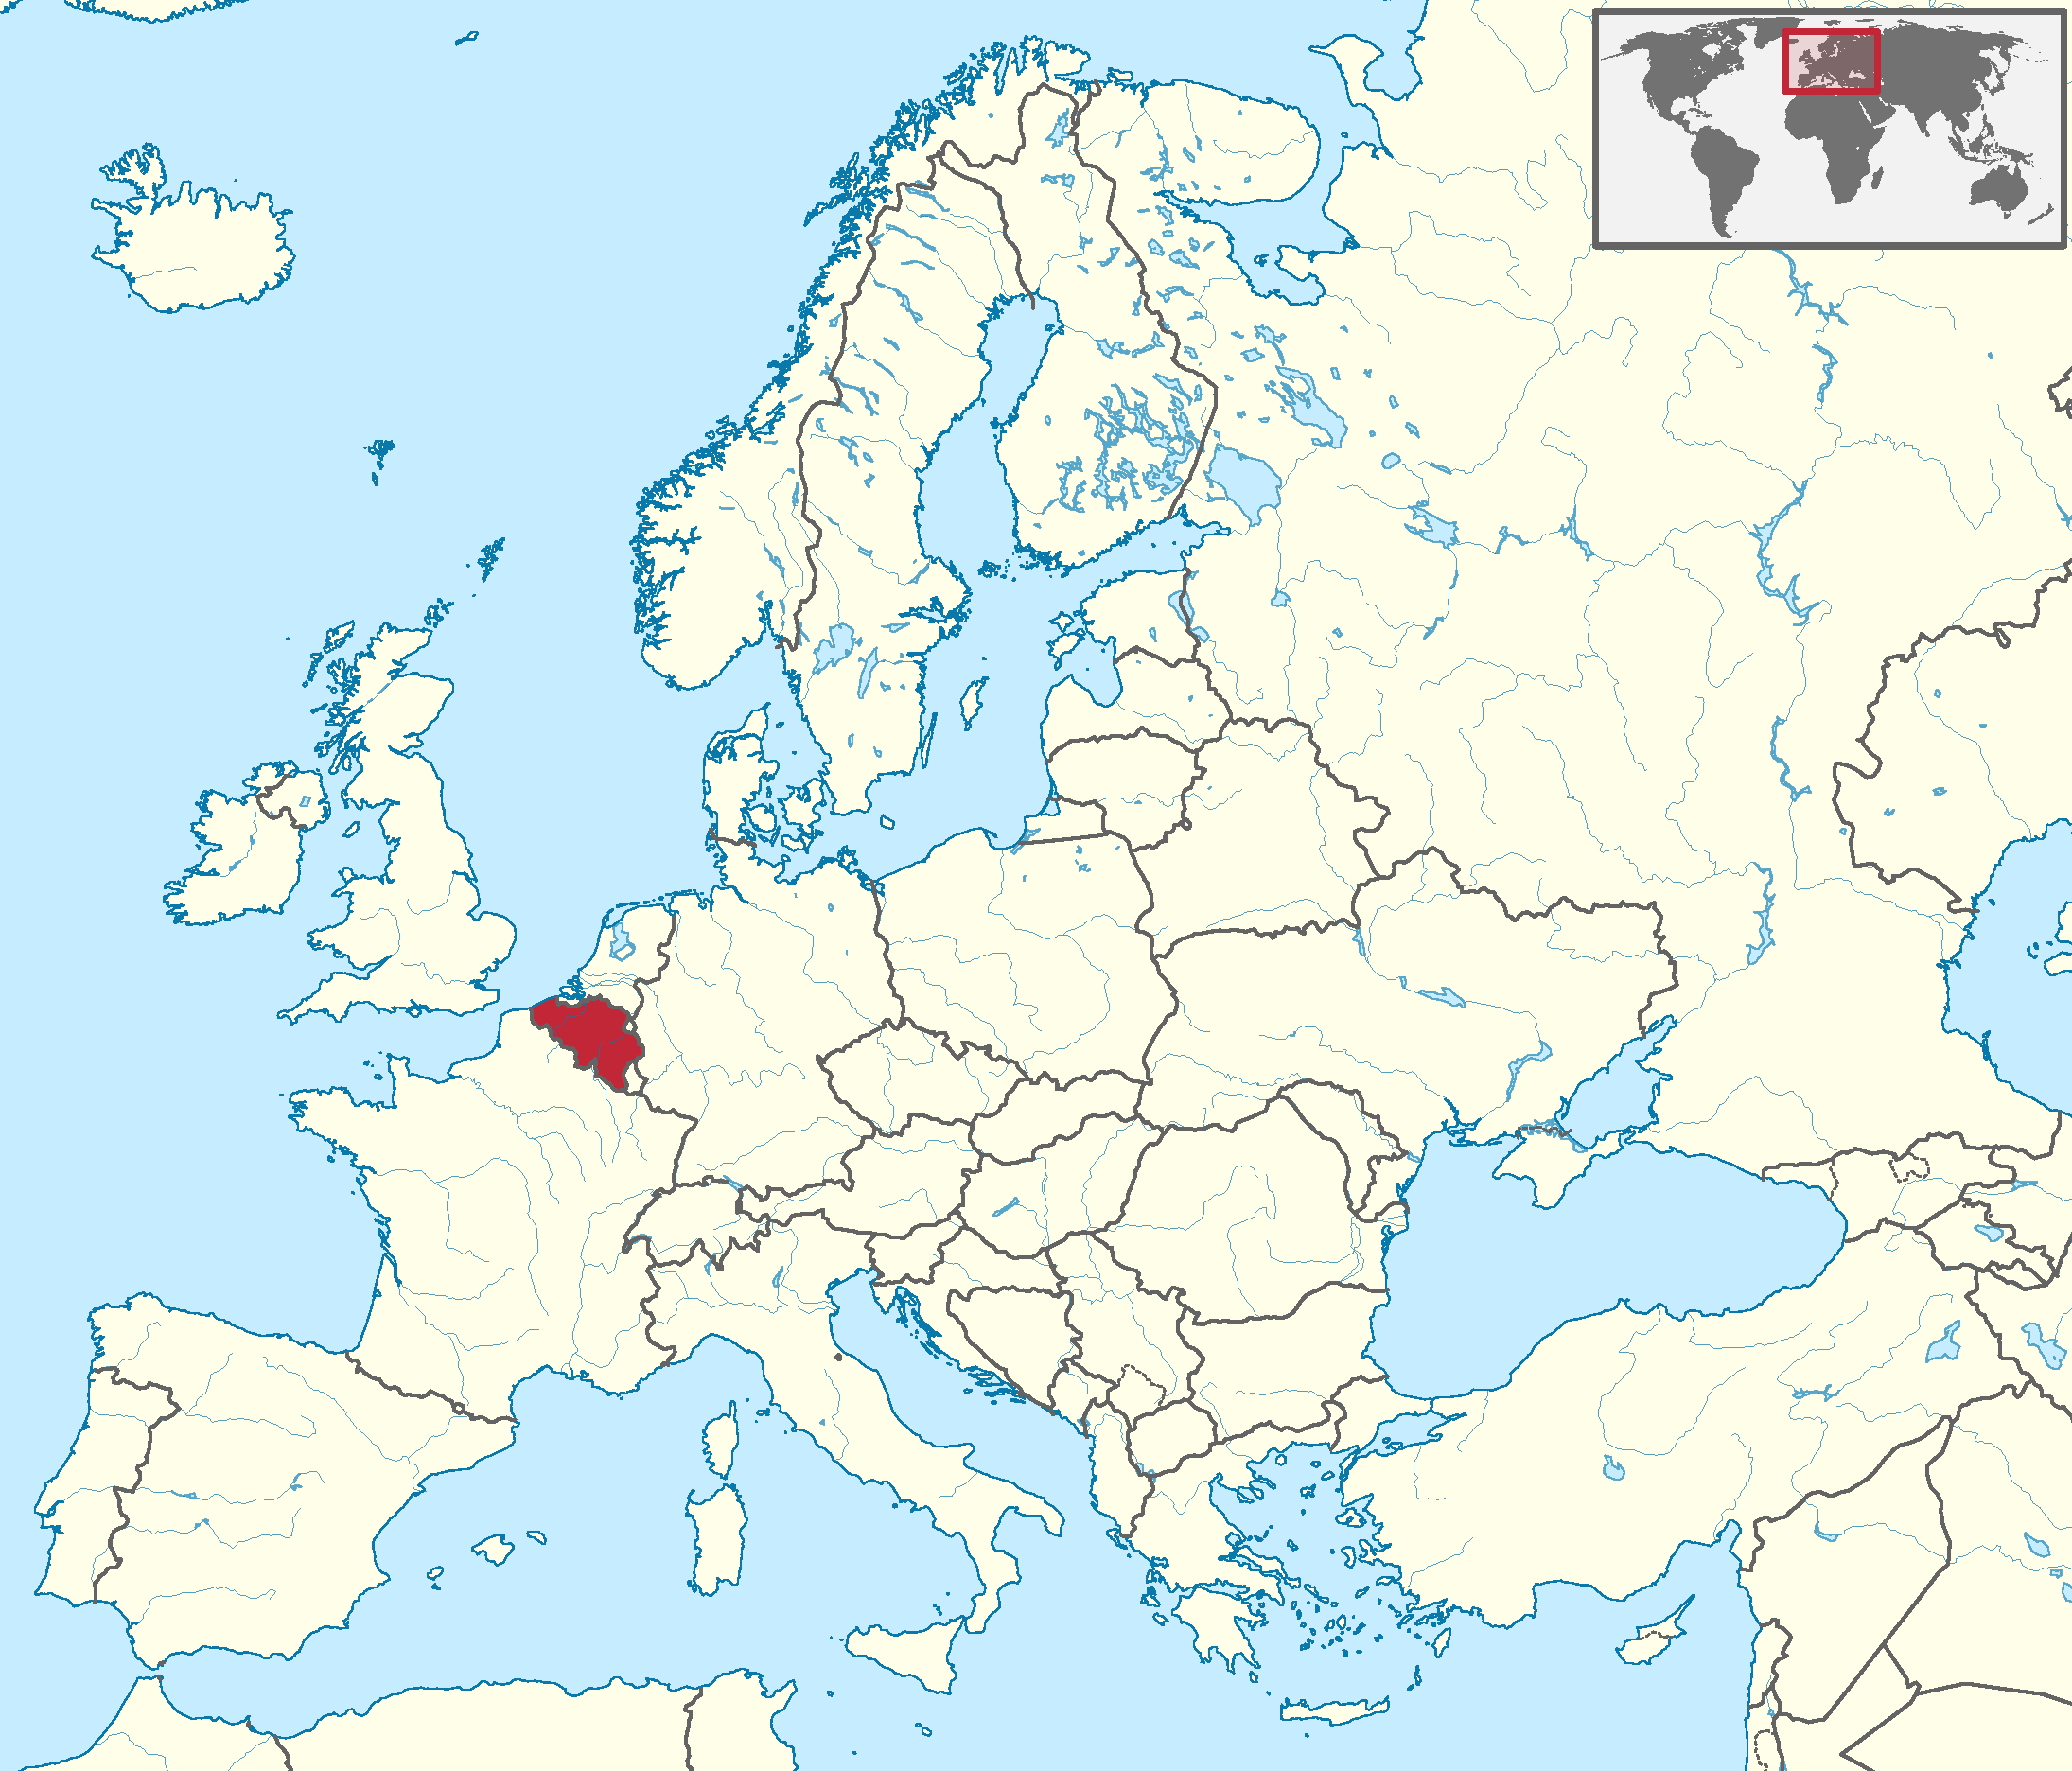
\includegraphics[width=\linewidth,height=0.68\textheight,keepaspectratio]{images/europe_map.pdf}
  \end{columns}
\end{frame}

% ------------------------------------------------------------------
\begin{frame}{Hobbies \& Interests \ja{趣味・関心}}
  \begin{columns}[T]
    \column{0.5\textwidth}
    \textbf{Sports \& Outdoors \ja{スポーツ・アウトドア}}
    \begin{itemize}
      \item Running, hiking, and exploring nature
      \item 6 years as a Scout Leader \ja{スカウトリーダー}
    \end{itemize}

    \vspace{6pt}
    \textbf{Culture \ja{文化・趣味}}
    \begin{itemize}
      \item Anime \& Manga enthusiast \ja{アニメ・マンガファン}
      \item Reading \& history
    \end{itemize}

    \column{0.5\textwidth}
    \textbf{Tech \& Coding \ja{技術・プログラミング}}
    \begin{itemize}
      \item Open-source software developer \ja{OSS開発}
      \item Contributor on GitHub \ja{GitHubでの活動}
      \item Passionate about Rust, Python, and JAX
    \end{itemize}

    \vspace{6pt}
    \textbf{Destination \ja{旅行}}
    \begin{itemize}
      \item Long-time dream: Visiting and working in Japan! \ja{日本での生活と研究}
    \end{itemize}
  \end{columns}
\end{frame}

\begin{frame}{Academic Supervisors\ja{指導教員}}
  \begin{columns}[c]
    \column{0.5\textwidth}
    \centering
    \includegraphics[height=2.5cm]{images/claude.jpeg}\\[2pt]
    \textbf{Prof.\ Claude Oestges} (UCLouvain)\\
    {\small Channel modeling, propagation, MIMO}

    \column{0.5\textwidth}
    \centering
    \includegraphics[height=2.5cm]{images/laurent.jpeg}\\[2pt]
    \textbf{Prof.\ Laurent Jacques} (UCLouvain)\\
    {\small Signal processing, computational sensing}
  \end{columns}
\end{frame}

% ==================== PART 2: WHAT DO I DO? ===========================
\section{\texorpdfstring{What I Do (Ph.D.\ Research) \ja{研究内容}}{What I Do}}

% ------------------------------------------------------------------
\begin{frame}{My Research Topic \ja{研究テーマ}}
  \begin{center}
    {\Large\bfseries Differentiable Ray Tracing \ja{微分可能レイトレーシング}\\for Radio Propagation Modeling \ja{電波伝搬モデリング}}
  \end{center}

  \vspace{10pt}

  \begin{columns}[c]
    \column{0.55\textwidth}
    \textbf{Key Concepts \ja{主要な概念}:}
    \begin{itemize}
      \item \textbf{Radio Propagation}: Model wireless signals in complex urban and indoor environments \ja{都市・室内での電波伝搬}
      \item \textbf{Ray Tracing}: Simulate physical wave interactions (reflections, diffractions) \ja{反射・回折の物理シミュレーション}
      \item \textbf{Differentiability}: Compute gradients through physics for fast gradient-based optimization \ja{勾配ベースの高速最適化}
    \end{itemize}

    \column{0.45\textwidth}
    \centering
    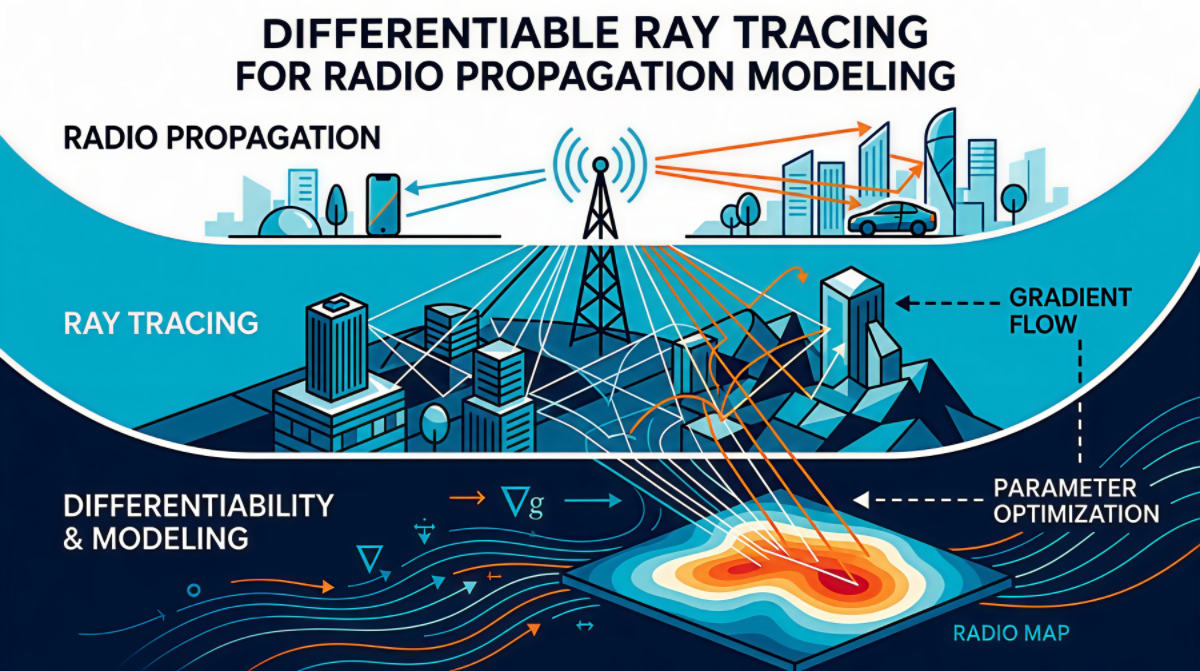
\includegraphics[width=\linewidth,keepaspectratio]{images/differentiable_ray_tracing.png}
  \end{columns}
\end{frame}

% ------------------------------------------------------------------
\begin{frame}{Key Highlight: Generative Path Sampling \ja{研究成果：生成型経路サンプリング}}
  \begin{columns}[c]
    \column{0.52\textwidth}
    \textbf{The Challenge \ja{課題}:}
    \begin{itemize}
      \item Point-to-point ray tracing requires searching $\mathcal{O}(N^K)$ candidate paths
      \item Exponential complexity \ja{計算量の指数関数的増大} limits real-time 5G/6G digital twin simulations \ja{デジタルツイン}
    \end{itemize}

    \vspace{4pt}
    \textbf{Our Solution \ja{解決策}:}
    \begin{itemize}
      \item Replace exhaustive search with an ML model (\textbf{GFlowNet}) \ja{強化学習・生成モデル}
      \item Samples physically valid paths directly
      \item \textbf{100$\times$ speedup on CPU}, \textbf{10$\times$ on GPU} \ja{大幅な高速化} while maintaining high accuracy ($>90\%$)
    \end{itemize}

    \column{0.48\textwidth}
    \centering
    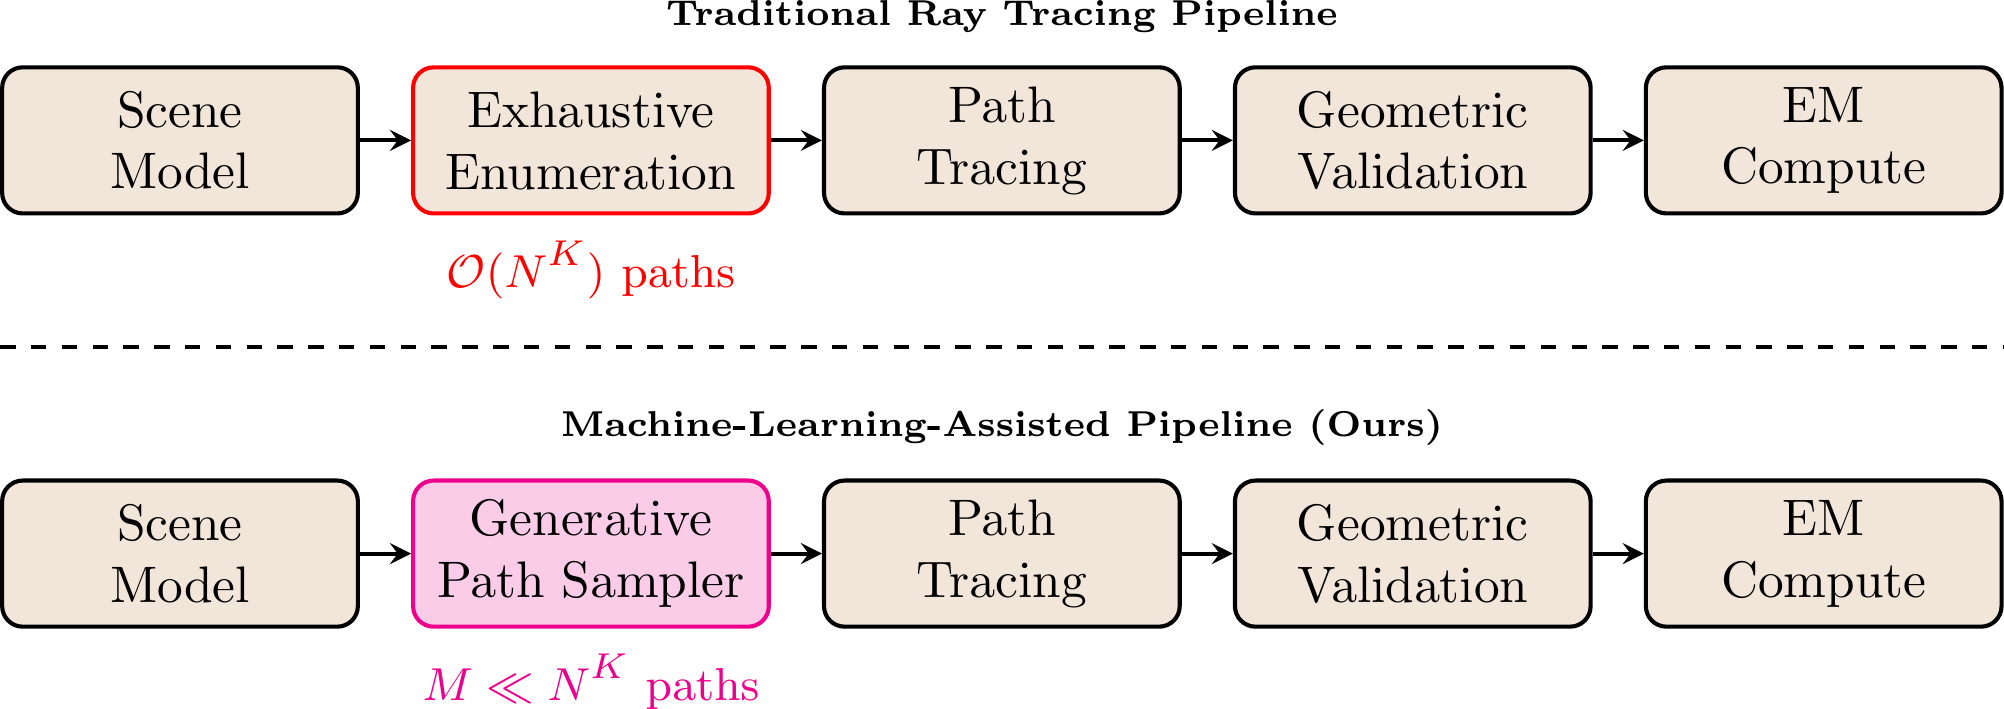
\includegraphics[width=\linewidth,height=0.65\textheight,keepaspectratio]{images/fig_pipeline.png}\\[2pt]
    {\footnotesize Traditional ray tracing (top) vs.\ ML-assisted path sampling (bottom)}
  \end{columns}
\end{frame}

% ------------------------------------------------------------------
\begin{frame}{Software \& Open-Source Projects \ja{開発ツール・成果物}}
  \begin{columns}[T]
    \column{0.5\textwidth}
    \textbf{DiffeRT \ja{微分可能レイトレーシング・ライブラリ}}
    \begin{itemize}
      \item Open-source Python library for differentiable radio ray tracing
      \item Built with JAX (GPU acceleration) \& Rust (high performance)
      \item {\small\url{https://github.com/jeertmans/DiffeRT}}
    \end{itemize}

    \column{0.5\textwidth}
    \textbf{Manim Slides \ja{プレゼンテーションツール}}
    \begin{itemize}
      \item Presentation tool for math \& scientific animations
      \item Used by researchers worldwide; published in JOSE journal
    \end{itemize}

    \vspace{6pt}
    \textbf{ADE Scheduler \ja{大学公式時間割システム}}
    \begin{itemize}
      \item University-wide course scheduling tool for UCLouvain (30k+ active student users)
    \end{itemize}
  \end{columns}
\end{frame}

% ==================== PART 3: WHY AM I HERE? ==========================
\section{\texorpdfstring{Why Am I Here? \ja{KDDI総合研究所での目標}}{Why Am I Here?}}

% ------------------------------------------------------------------
\begin{frame}{Why KDDI Research, Inc. \& Internship Goals \ja{KDDI総合研究所での研究目標}}
  \begin{columns}[T]
    \column{0.5\textwidth}
    \textbf{Why KDDI Research? \ja{志望理由}}
    \begin{itemize}
      \item Leading global telecommunications operator \ja{通信分野の世界的リーダー}
      \item Strong alignment with 5G/6G channel modeling, digital twins, and AI-driven network planning
      \item Opportunity to bring academic differentiable ray tracing to industrial applications \ja{産業応用への展開}
    \end{itemize}

    \column{0.5\textwidth}
    \textbf{Internship Goals \ja{インターンシップの目標}}
    \begin{itemize}
      \item \textbf{Professional}: Collaborate with KDDI researchers and produce high-impact R\&D results
      \item \textbf{Personal}: Improve Japanese language skills, experience Japanese work culture, and build lasting connections
    \end{itemize}
  \end{columns}
\end{frame}

% ------------------------------------------------------------------
\begin{frame}{}
  \vfill
  \begin{center}
    {\Huge\bfseries Thank you!}\\[12pt]
    {\Large ご清聴ありがとうございました}\\[18pt]
    {\large Jérome Eertmans}\\[6pt]
    {\small
      \href{https://eertmans.be}{eertmans.be}
      \quad$\cdot$\quad
      \href{https://github.com/jeertmans}{github.com/jeertmans}
      \quad$\cdot$\quad
      \href{mailto:jeertmans@icloud.com}{jeertmans@icloud.com}
    }
  \end{center}
  \vfill
\end{frame}

% ==================================================================
%  APPENDIX / BACKUP SLIDES (FOR Q&A SESSION)
% ==================================================================
\appendix
\sectionslide{Appendix / Backup Slides \ja{補足資料}}

% ------------------------------------------------------------------
\begin{frame}{Backup: Generative Path Sampling Architecture \ja{補足：モデル構成}}
  \centering
  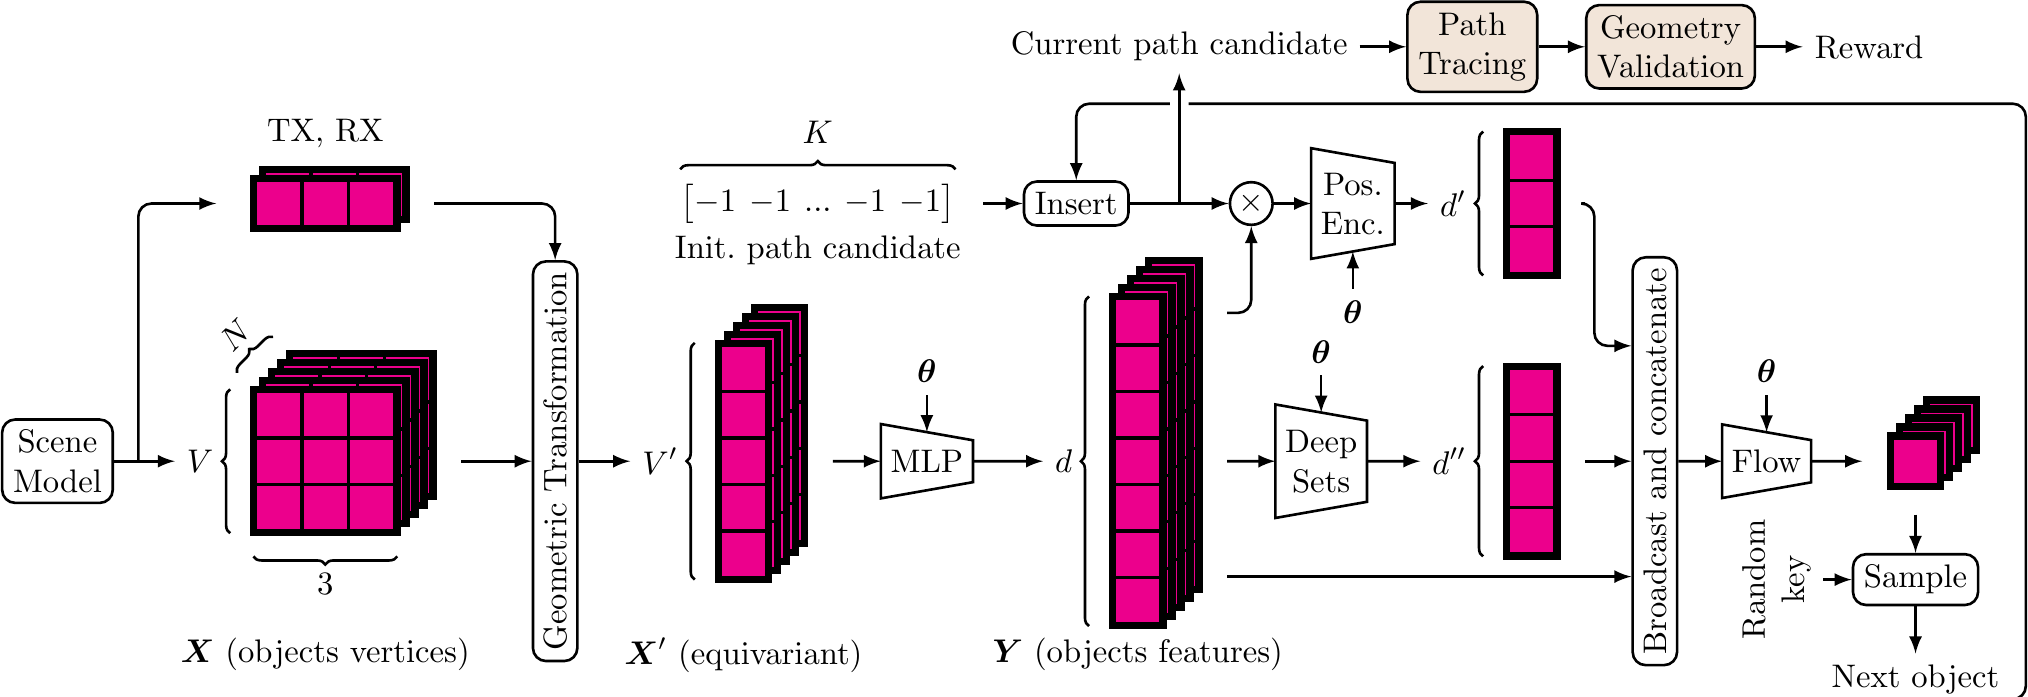
\includegraphics[width=0.88\textwidth,height=0.45\textheight,keepaspectratio]{images/fig_model.png}\\[3pt]

  \begin{columns}[T]
    \column{0.5\textwidth}
    {\small
    \begin{itemize}\itemsep2pt
      \item \textbf{GFlowNet} trained to sample promising ray paths
      \item Canonical transformation for spatial invariance
    \end{itemize}}

    \column{0.5\textwidth}
    {\small
    \begin{itemize}\itemsep2pt
      \item Physics-based action masking to eliminate invalid reflections
      \item Robust training via experience replay buffer
    \end{itemize}}
  \end{columns}
\end{frame}

% ------------------------------------------------------------------
\begin{frame}{Backup: Manhattan Benchmark Results \ja{補足：Manhattan都市モデル評価}}
  \begin{columns}[c]
    \column{0.55\textwidth}
    \centering
    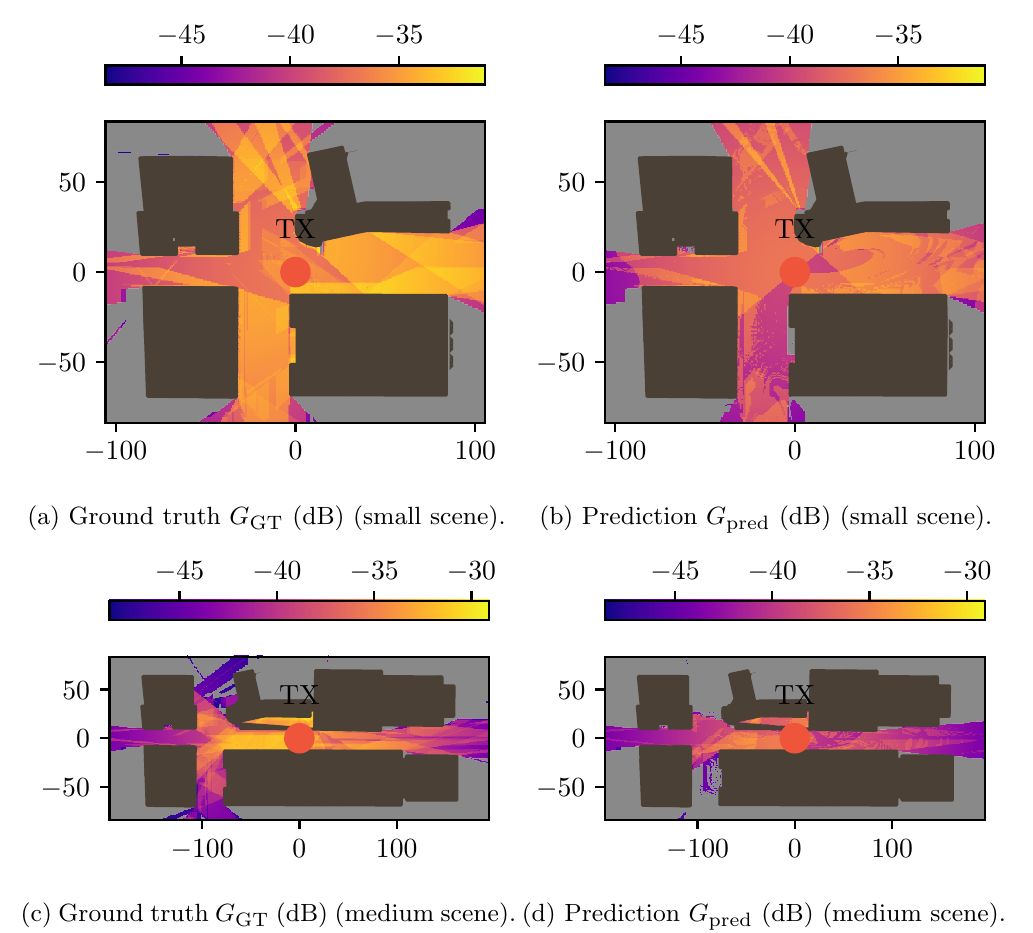
\includegraphics[width=\linewidth,height=0.75\textheight,keepaspectratio]{images/fig_coverage_manhattan.png}

    \column{0.45\textwidth}
    \textbf{Out-of-Distribution Generalization \ja{汎化性能}}
    \begin{itemize}\itemsep4pt
      \item Trained on street canyons, tested on real OpenStreetMap Manhattan geometry ($N$ up to 805 objects)
      \item Captures dominant propagation channels efficiently
    \end{itemize}
  \end{columns}
\end{frame}

% ------------------------------------------------------------------

\end{document}
